\section{Smooth distance functions}
In this section, we study specific distance functions that satisfy the triangle inequality. One such family is the space of metrics on a given sample space $\cX$. We consider these specific distance functions and establish the framework for oblivious teaching, achieving an error bound of \(\epsilon > 0\) on all possible triplet comparisons. This is achieved under certain mild assumptions regarding the underlying distance function and the distribution over the input space \(\cX\), as outlined in the preceding discussion.

Consider general distance functions defined on a separable metric space \((\cX, d)\), where \(\cX \subset \mathbb{R}^k\) is a compact set, which means it is both closed and bounded within \(\mathbb{R}^k\). The distance function \(d: \cX \times \cX \to \mathbb{R}^{+}\) is assumed to be a \(C^2\)-map with respect to each argument (with symmetry of \(d\) implying this smoothness in both arguments). 

To effectively teach the distance function \(d\), the teacher employs a dual strategy that combines \texttt{local} and \texttt{global} distance approximations. The global approximation is achieved through a finite-sample distance function, while local approximations leverage Mahalanobis distance metrics, derived from the curvature information of a local neighborhood through its Hessian (see \figref{fig:bothfigures} for an illustration).

\paragraph{Local approximations:} Local approximation of the distance function $d$ is based on the taylor series expansion around the neighborhood at a given point. First, we state a high-dimensional version of Taylor's formula:
\begin{theorem}[Theorem 2.6.8~\citet{folland2002advanced}]\label{thm:taylorseries}
Suppose \( f : \mathbb{R}^k \rightarrow \mathbb{R} \) is of class \( C^{k+1} \) on an open convex set \( S \).
If \( a \in S \) and \( a + \mathbf{h} \in S \), then
\begin{equation}
f(a + \mathbf{h}) = \sum_{|\alpha| \leq k} \frac{\partial^\alpha f(a)}{\alpha!} \mathbf{h}^\alpha + R_{a,k}(\mathbf{h}),
\end{equation}
where
\begin{equation}
R_{a,k}(\mathbf{h}) = \sum_{|\alpha| = k+1} \frac{\partial^\alpha f(a + c\mathbf{h})}{\alpha!} \mathbf{h}^\alpha \quad \text{for some } c \in (0, 1). \label{eq: rem}
\end{equation}
%\begin{equation}
%R_{a,k}(\mathbf{h}) = k \sum_{|\alpha| = k} \frac{\mathbf{h}^\alpha}{\alpha!} \int_0^1 (1 - t)^{k-1} %\left[\partial^\alpha f(a + t\mathbf{h}) - \partial^\alpha f(a)\right] dt.
%\end{equation}
%If \( f \) is of class \( C^{k+1} \) on \( S \), we also have
%\begin{equation}
%R_{a,k}(\mathbf{h}) = (k + 1) \sum_{|\alpha| = k+1} \frac{\mathbf{h}^\alpha}{\alpha!} \int_0^1 (1 - t)^k \partial^\alpha f(a + t\mathbf{h}) dt,
%\end{equation}
%and
%\begin{equation}
%R_{a,k}(\mathbf{h}) = \sum_{|\alpha| = k+1} \frac{\partial^\alpha f(a + c\mathbf{h})}{\alpha!} \mathbf{h}^\alpha \quad \text{for some } c \in (0, 1). \label{eq: rem}
%\end{equation}
\end{theorem}

%\begin{theorem}[Taylor's expansion for Banach space, Page-%276,~\cite{Planitz_1980}]\label{thm:taylorseries}
%    Let $X, Y$ be two Banach spaces, $U$ open in $X$, and $x$ a point of $X$. Let $F: U \to Y$ be such that $\partial_x F$ is Frechet differentiable. Then for all $h \in U$, we have
%\[
%F(x + h) = F(x) + \frac{F'(x)h}{1!} + \frac{1}{2}\curlybracket{F''(x)h}h + o(||h||^2)
%\]

%\end{theorem}

\begin{figure}[t]
    \centering
    \begin{subfigure}[b]{0.45\textwidth}
        \centering
        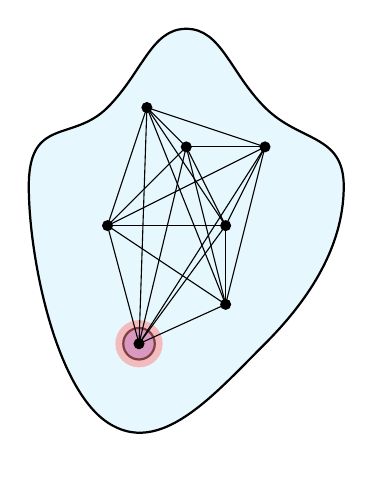
\begin{tikzpicture}
            \begin{scope}[]

            
                 \fill[cyan!10] plot [smooth cycle, tension=0.8] coordinates {(1,3) (0,2) (-1,1) (0,-2) (2,-1) (3,1) (2,2)};
            
            % Draw the outer shape
            \draw[thick] plot [smooth cycle, tension=0.8] coordinates {(1,3) (0,2) (-1,1) (0,-2) (2,-1) (3,1) (2,2)};
        
            % Fill the i\sf{NN}er circle
            \fill[blue!30] (0.4, -1.0) circle (0.2);
            
            % Draw the i\sf{NN}er circle with edges
            \draw[thick] (0.4, -1.0) circle (0.2);
        
            % Draw and fill another circle without edges
            \fill[red!50, opacity=0.5] (0.4, -1.0) circle (0.3);
            
            % Define the coordinates of the vertices
            \coordinate (A) at (0, 0.5);
            \coordinate (B) at (1, 1.5);
            \coordinate (C) at (1.5, 0.5);
            \coordinate (D) at (2, 1.5);
            \coordinate (E) at (0.5, 2);
            \coordinate (F) at (1.5, -0.5);
            \coordinate (G) at (0.4, -1.0);
        
            % Draw the vertices
            \foreach \i in {A, B, C, D, E, F, G} {
                \fill (\i) circle (2pt);
            }
        
            % Draw the edges
            \foreach \i/\j in {A/B, A/C, A/D, A/E, A/F, B/C, B/D, B/E, B/F, B/G, C/D, C/E, C/F, C/G, D/E, D/F, D/G, E/F, E/G, F/G} {
                \draw (\i) -- (\j);
            }
            \draw (A) -- (G);
            \end{scope}
        \end{tikzpicture}
        \caption{Global approximation using a finite-sample distance function}
        \label{fig:figure1}
    \end{subfigure}
    %\hfill
    \begin{subfigure}[b]{0.45\textwidth}
        \centering
        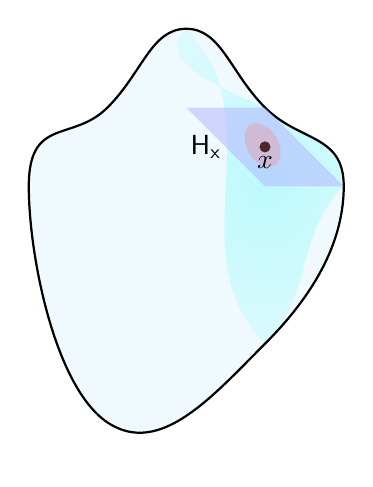
\begin{tikzpicture}
            \begin{scope}[]
    % Define the coordinates of the outer shape
    %\path[name path=shape] plot [smooth cycle, tension=0.8] coordinates {(3,4) (2,3) (1,2) (2,-1) (4,0) (5,2) (4,3)};

    % Define the shading
    \begin{scope}
        \clip plot [smooth cycle, tension=0.8] coordinates {(3,4) (2,3) (1,2) (2,-1) (4,0) (5,2) (4,3)};
        \shade[inner color=cyan!50, outer color=cyan!20] (3,4) to[out=-45, in=135] (4,0) to[out=45, in=-135] (5,2) to[out=45, in=225] cycle;
    \end{scope}
    \fill[cyan!10,opacity=.6] plot [smooth cycle, tension=0.8] coordinates {(3,4) (2,3) (1,2) (2,-1) (4,0) (5,2) (4,3)};
    % Draw the outer shape outline
    \draw[thick] plot [smooth cycle, tension=0.8] coordinates {(3,4) (2,3) (1,2) (2,-1) (4,0) (5,2) (4,3)};

    % Define the coordinates of the parallelogram
    \coordinate (A) at (4,2);
    \coordinate (B) at (5,2);
    \coordinate (C) at (4,3);
    \coordinate (D) at (3,3);

    % Draw the parallelogram
    %\draw[thick] (A) -- (B) -- (C) -- (D) -- cycle;

    
    % Draw the tangent rectangle
    \fill[blue!30,opacity=.5] (A) -- (B) -- (C) -- (D) -- cycle;
    %\draw[thick] (3,2) rectangle (5,3);
    
    % Draw the point inside the rectangle
    \fill[black] (4, 2.5) circle (2pt);

    \fill[red!50, opacity=0.3, rotate=30] (4.7, 0.2) ellipse[x radius=0.2, y radius=0.3];

    \node at (3.25, 2.5) {$\sf{H}_x$};
    \node at (4, 2.3) {$x$};
\end{scope}
        \end{tikzpicture}
        \caption{Linear approximation at $x$: $\sf{H}_x$}
        \label{fig:figure2}
    \end{subfigure}
    \caption{Approximation of the metric $d$: Linear and Finite-sample approximations}
    \label{fig:bothfigures}
\end{figure}

We are interested in using \thmref{thm:taylorseries} to devise local linear approximation to $d$.
Consider the following:
\begin{align*}
    d(x,x') = d(x,x) + (x'-x)^{\top}\cdot\boldsymbol{\partial}_{x} d(x,\cdot) + \frac{1}{2!}(x'-x)^{\top} \sf{H}_x d(x,\cdot) (x'-x) + R_{x,3}(x'-x)
\end{align*}
Here, we assume that for all $\alpha \in [n]^3$, the partial derivative is bounded, i.e $|\partial^\alpha d(x,\cdot)| \le M$ for some constant $M > 0$. Thus, the remainder term $R_{a,k}(\mathbf{h})$ in \eqnref{eq: rem} can be bounded as 
\begin{align*}
 |R_{a,k}(\mathbf{h})| = \bigg\lvert\sum_{|\alpha| = k+1} \frac{\partial^\alpha f(a + c\mathbf{h})}{\alpha!} \mathbf{h}^\alpha\bigg\rvert \le \frac{M n^{\frac{k+1}{2}}}{(k+1)!} \cdot||\mathbf{h}||^{k+1}_2   
\end{align*}

Since $d$ is a metric it is straightforward to note that $\boldsymbol{\partial}_{x} d(x,\cdot) = 0$. Now, if $||x'-x|| \le \xi$, we have
\begin{subequations}\label{eq: 1}
\begin{align}
    d(x,x') &= \frac{1}{2!}(x'-x)^{\top} \sf{H}_x d(x,\cdot) (x'-x) + \Tilde{O}(||x'-x||_2^{2})\\
    \implies d(x,x') &\approx_{\xi} \frac{1}{2!}(x'-x)^{\top} \sf{H}_x d(x,\cdot) (x'-x)
\end{align}
\end{subequations}
So, for all distances centered at $x$ the inner product $(x'-x)^{\top} \sf{H}_x d(x,\cdot) (x'-x)$ is a tight linear approximation to $d$ with error at most $\xi^2$ within a ball of norm up to $\xi$. Note that since $d(x,\cdot)$ is a convex function at $x$ the hessian operator $\sf{H}_x$ is positive semi-definite. Since it is symmetric, we obtain a local Mahalanobis distance at $x$ in a $\xi$ neighborhood around $x$.

Now, we note a simple observation for this local approximation, i.e. 
\begin{align}
    (x'-x)^{\top} \sf{H}_x d(x,\cdot) (x'-x) \le \gamma_{\max}\cdot ||x-x'||_2^2 \label{eq: mahaapp}
\end{align}
Thus, if $\ell_2$ norm of two samples is small, so is the local approximation wrt the Mahalanobis distance function with matrix $\sf{H}_x$.

\paragraph{Global approximation:} Now, we will discuss the global approximation of the distance function $d$ using a finite sample distance function. Given that $\cX$ is a compact separable space, there is a finite $\epsilon$-cover of the space for any $\epsilon > 0$. Consider an $\epsilon$-cover $\cC_{\cX} \subset \cX$ (denoted $\cC$ for ease of notation) such that for all $x \in \cX$
\begin{align*}
    \exists c \in \cC, d(x,c) \le \epsilon %\cC_{\cX} =  \curlybracket{B_d(x,\epsilon) \,|\, x \in \cC}
\end{align*}
Note that, $\cX \subset {\bigcup}_{x \in \cC} B_d(x,\epsilon)$. We can similarly define an $\epsilon$ cover for $\ell_2$ distance as well. Later in the section we discuss an approximation method via $\ell_2$ cover of the space $\cX$.
%\sanjoy{This notation, which differentiates $\cC$ from $\cC$, is a bit cumbersome. Maybe we can just let $\cC$ be the centers of the covering balls (i.e. what $\cC$ is)?}

Note that the teacher can exactly specify the distances on $\cC$ wrt $d$ upto triplet comparisons as $d_G$, i.e.
\begin{align*}
    \forall x, x',x'' \in \cC,\,\, (x,x',x'')_{d_G} \,\,\textit{iff}\,\, (x,x',x'')_{d}
\end{align*}
For the study here, we assume the sample space is continuous. Thus, in order to analyze the performance of a taught metric $d'$ we define a notion of \tt{regret}, denoted as $\cR$, for a learner making mistakes in providing the correct relation on the comparisons on a given triplet $(x, x',x'')$ using $d'$ against the target metric $d$ as follows:
\begin{align*}
    \cR_{d'}(x, x',x'') = \begin{cases}
        0 & \textnormal{if } (x, x',x'')_{d'} = (x, x',x'')_{d}\\
        1 & \textnormal{o.w.}
    \end{cases}
\end{align*}
Here, we abuse the notation, alternately assume that $(x, x',x'')_{d'}$ means $d'$ assigns a comparison over $x,x',x"$, in addition to the usual understanding that $d'(x,x') \ge d'(x,x")$.

\textbf{Remark.} \tt{We assume that, in order to break ties among equal distances, the teacher could provide a triplet $(x,y,z)$ with the signal if there is equality or inequality, i.e. $d(x,y) = d(x,z)$ or $d(x,y) > d(x,z)$. We need this strong triplet comparison so that the learner can distinguish if the distances are equal or not, in the absence of which, it could choose a degenerate metric with all the distances equal.}

Now, we are interested in how good is $d'$ compared to $d$ which we measure in terms of $\epsilon$-error defined as follows: 
\begin{definition}
    For a given metric $d$, we say an approximation $d'$ achieves $\epsilon$-error against $d$ if 
    there exists a constant $C > 0$ such that
\begin{align*}
    \expctover{(x,y,z) \sim \cX^3}{\cR_{d'}(x,y,z)} \le C\cdot\epsilon
\end{align*}
    
\end{definition}
We assume the realizable case and thus $d$ has $0$ error on the sample space. 

Before we state our main result of the section, we consider a regularity condition of smoothness on the given distribution $\mu$ over the sample space $\cX$. 


\begin{definition}[Lipschitz smoothness of $\mu$]\label{def: lipschitz} We say a distribution $\mu$ over a metric space $(\cX,d)$ is $L$-Lipschitz smooth if there exists a parameter $\alpha > 0$ such that the following property holds on open normed balls:
\begin{align*}
    \forall x \in \cX,\,\, \forall r,r' > 0, \,\, |\mu(B_2(x,r)) - \mu(B_2(x,r'))| \le L \cdot |r - r'|^{\alpha}
\end{align*}
where $B_2(x,r) := \curlybracket{x' \in \cX\,|\, ||x - x'||_2 \le r}$.
\end{definition}
An implication of this definition is
\begin{align}
    &\liminf_{r_n \downarrow 0} |\mu(B_2(x,r)) - \mu(B_2(x,r_n))| \le \liminf_{r_n \downarrow 0} L \cdot |r - r_n| \nonumber\\
    \implies & \mu(B_2(x,r)) - \liminf_{r_n \downarrow 0} \mu(B_2(x,r_n)) \le L\cdot r^\alpha \nonumber\\
    \implies & \mu(B_2(x,r)) \le L\cdot r^\alpha \label{eq: rbound}
\end{align}

\subsection{Naive approximation of a smooth distance function via $\ell_2$ distance function}
%\sanjoy{I think there should be two results. The first should just say that any triplet $(x,y,z)$ is answered correctly if $d(x,y) - d(x,z) > \epsilon$. The second can be a distributional corollary. The theorem statement for the first should include all assumptions about the distance functions, e.g. that the third partial derivatives are uniformly bounded by $M$ and that all Hessians have maximum eigenvalue bounded by $\gamma$. The number of triplets needed can then be given explicitly in terms of an $\ell_2$ covering number of $\cX$, with radius in terms of $\epsilon, M, \gamma$ and whatever else.}
\paragraph{Distance Model:} In this section, we consider a model $\cM = \curlybracket{(\cC, d_{\cC}, \ell_2)}$ where $\cC \subset \cX$ of finite cardinality and $d_{\cC}: \cC \times \cC \to \reals_{+}$ is finite-sample distance function on $\cC$. Any distance function $d \in \cM$ has the following form:
\begin{equation*}
    d(x,y) = d(c(x), c(y)) 
\end{equation*}
where $c(x) = \argmin_{c \in \cC} ||c - x||_2$.

\begin{theorem}\label{thm: smoothl2} Consider a compact separable metric space $\cX \subset \reals^k$. Consider a distance function $d: \cX \times \cX \to \reals_{\ge 0}$ that is a $C^2$-map in the second argument. Assume that $d$ satisfies the following properties:
\begin{enumerate}
    \item it satisfies the triangle inequality\footnote{Since we needn't have symmetric $d$ note the directional version of this triangle inequality which is consistent with the parallelogram law of vector addition.} over $\cX$, i.e. for all $x,y,z \in \cX$, $d(x,y) + d(y,z) \ge d(x,z)$,
    \item it has uniformly bounded third partial derivative by a constant $M > 0$, and
    \item at any sample $x \in \cX$, $\lambda_{\max}(\sf{H}_x d(x,\cdot))$ is bounded by a constant $\gamma > 0$. 
\end{enumerate}

%Consider a distribution $\mu$ over $\cX$ which is $L$-lipschitz. %for some constant $\frac{1}{\lambda_{\textsf{diam}}}\ge L > 0$ where $\lambda_{\textsf{diam}} = \textsf{diam}(\cX)$. 
Then, for any error parameter $\epsilon > 0$, there exists a finite-sample distance function $d'$ (see \algoref{alg: smoothdistl2}) which can be taught with $\cN(\cX, \epsilon(\epsilon, M, \gamma), \ell_2)^2$ triplet comparisons such that for any $x,y,z \in \cX$, if $d(x,y) > d(x,z) + \epsilon$ then
\begin{align*}
    d'(x,y) > d'(x,z)
\end{align*}
where the covering accuracy $\epsilon(\epsilon, M, \gamma)$ denotes that the covering depends on $\epsilon$, and constants $M$ and $\gamma$.

%there exists a distance function $d'$ which can be taught with $\cN(\cX, \epsilon)^2$ triplet comparisons such that 

%achieving an $\epsilon$-error, i.e. there exists a constant $C > 0$ such that
%\begin{align*}
%    \expctover{(x,y,z) \sim \cX^3}{\cR_{d'}(x,y,z)} \le C\cdot\epsilon
%\end{align*}
    
\end{theorem}
\begin{algorithm}[t]
\caption{Teaching a smooth distance function with $\ell_2$ covering of the space}
\label{alg: smoothdistl2}
\textbf{Given}: Input space $\cX \sim \cC_{\cX}$, error threshold: $\epsilon$.\\
\vspace{1mm}
\textit{In batch setting:}\vspace{1mm}
\begin{enumerate}
    \item teacher provides triplet comparisons $\cT$ corresponding to finite-sample distance function $(\cC, d)$ for an $\epsilon$-cover $\cC_2(\cX,\epsilon,\ell_2)$.
\end{enumerate}
For a given sample $x$, learner computes:
\begin{itemize}
    \item $\cC_x := \curlybracket{c \in \cC: ||x - c ||_2 \le \epsilon}$ 
    \item $c_x := \argmin_{c \in \cC_x} \sqrt{(x-c)^{\top}(x-c)}$
\end{itemize}
\vspace{1mm}
To answer query on $(x,y,z)$, learner checks:
\begin{itemize}
    \item \textbf{If} $c_y = c_z$, then say $``d(x,y) \approx d(x,z)"$
    \item \textbf{Else}: answer according to the triplet $(c_x,c_y,c_z)$.
\end{itemize}
\end{algorithm}

\begin{proof}
    The proof requires a global approximation using an $\epsilon$-cover wrt $\ell_2$ distance.
    
   Consider an $\epsilon$-cover $\cC(\cX,\epsilon,\ell_2)$, denoted as $\cC_2(\cX)$ (in short) with centers $\cC$. The teacher provides triplet comparisons to teach a finite-sample distance function $(\cC, d)$, with the underlying distance function denoted as $d_G$ such that
        \begin{align*}
            x,y,z \in \cC,\quad (x,y,z)_{d_G} \textit{ iff } (x,y,z)_{d}
        \end{align*}
        For oblivious teaching,  $\cC_2(\cX)^2$ (square of covering number) many triplet comparisons are sufficient to teach $d_G$.
      %  \item[ii)] \tt{Local approximation:} For each center $x \in \cC$, consider local linear approximations $\sf{H}_x d$ with error bounded by $\xi$ where $\xi \le \frac{\epsilon}{6}$ (see \eqnref{eq: 1}). For each hessian operator $\sf{H}_x$, teacher provides triplets based on its eigendecompositon as discussed in previous sections. Each linear transformations requires at most $n^2$ (where $n$ is the ambient space dimension) many triplets. We use the notation $\hat{\sf{H}}_x$ for a taught matrix against the correct hessian matrix $\sf{H}_x$ for any $x \in \cX$. 

    Now, we discuss how a learner assigns comparisons for $d'$ for a given triplet $(x_1,x_2,x_3) \in \cX^3$. Denote by $\sf{NN}_2: \cX \to \cX$, a nearest neighbor map based on $\ell_2$ distances of any sample $x \in \cX$ (from the centers $\cC$). Thus, 
    \begin{align*}
        \sf{NN}_2(x) = \argmin_{x' \in \cC} \sqrt{(x-x')^{\top}(x-x')}
    \end{align*}
    We break the ties arbitrarily. This could potentially create some error in assigning the right comparison, which would at the worst only add a constant multiple of $\epsilon$ on the error. Denote by $\hat{x}$, the nearest neighbor of $x \in \cX$, i.e.  $\hat{x} \in \sf{NN}_2(x)$.
    $d'$ assigns the comparison on the triplet $\hat{x}_1, \hat{x}_2,\hat{x}_3$ as follows:
    %Now, the learner constructs a metric $d'$ to assign relation on any arbitrary triplet $(x_1,x_2,x_3) \in \cX^3$ as follows: %(this could be extended to quadruples similarly):
    %\begin{align}
    %    d'(x_1,x_2) \ge d'(x_1,x_3) = (\sf{NN}(x_1), \sf{NN}(x_2), \sf{NN}(x_3))_{d_G} \label{eq: assign}
    %\end{align}
    %Here, $\sf{NN}$ denotes the nearest neighbor based on local linear approximations. In the \eqnref{eq: assign} above, we assume that $\sf{NN}(x_2)$ is closer to $\sf{NN}(x_1)$ than $\sf{NN}(x_3)$, otherwise the relation could be written accordingly.
    %There are two possibilities for the 
    \begin{align}\label{eq: approxmetric}
        (x_1,x_2,x_3)_{d'} = \begin{cases}
            (\hat{x}_1,\hat{x}_2,\hat{x}_3)_{d_G} & \textit{ if } 
            \hat{x}_1 \neq \hat{x}_2 \textit{ or } \hat{x}_1 \neq \hat{x}_3\\
            d'(x_1,x_2) = d'(x_1,x_3)  & \textit{ o.w. }   %\hat{x}_1 = \hat{x}_2 = \hat{x}_3       \textit{ and } ({x}_1 -  {x}_2) \hat{\sf{H}}_{x_1}({x}_1 -  {x}_2)^{\top} \ge ({x}_1 -  {x}_3) \hat{\sf{H}}_{x_1}({x}_1 -  {x}_3)^{\top}
            %(\hat{x}_1,\Hat{x}_3,\hat{x}_2)_{d_{\sf{local}}}  & \textit{ if }   \hat{x}_1 = \hat{x}_2 = \hat{x}_3       \textit{ and } ({x}_1 -  {x}_3) \hat{\sf{H}}_{x_1}({x}_1 -  {x}_3)^{\top}  \ge   ({x}_1 -  {x}_2) \hat{\sf{H}}_{x_1}({x}_1 -  {x}_2)^{\top}
        \end{cases}
    \end{align}
    %where $d_{\sf{local}}$ is written as an abuse of notation for $d_{\hat{\sf{H}}_x}$ for any $x \in \cX$. 
    
     So, the learner answers: if ``$x_2$ is closer to $x_1$ than $x_3$'' by first finding the nearest neighbors of these points and then checking the corresponding relation to these in the distance function $(\cC, d_G)$. %and local Mahalanobis metrics induced by $\{\hat{\sf{H}}_x: x \in \cC\}$.
     Thus, the distance function $d'$ is defined as follows: for all $x,y \in \cX$
     \begin{equation}
         d'(x,y) := d_G(\hat{x}, \hat{y})
     \end{equation}
    Now, we will show the approximation guarantee for $d'$.
    
    First, we define the following maximum over the largest eigenvalues of the hessian operators $\curlybracket{\sf{H}_x}_{x \in \cC}$
\begin{align*}
    \hat{\gamma} := \max_{x \in \cC} \gamma_{\max}(\sf{H}_x)
\end{align*}
    
    Note, that the specific choice of the cover $\cC_2(\cX)$, and local approximations in \eqnref{eq: 1} and \eqnref{eq: mahaapp}
    %of the approximation constant $\xi$ for local approximation in ii), 
    ensures that if any points $y,z$ are far apart wrt a given $x$ then the distances are correctly captured, i.e. for any $x,y \in \cX$:
    \begin{align}
        d(x,y) - 2\hat{\gamma}\epsilon - 2\xi \le d(\hat{x}, \hat{y}) \le  d(x,y) + 2\hat{\gamma}\epsilon + 2\xi \label{eq: apdist}
    \end{align}
    We can show this as follows. Using triangle inequality we have
    \begin{align*}
        d(x,y) \le d(\hat{x},y) + d(\hat{x},x)\\
        d(\hat{x},y) \le d(\hat{x},\hat{y}) + d(\hat{y},y)
    \end{align*}
    Summing these 
    \begin{align}
        d(x,y) \le d(\hat{x},\hat{y}) + d(\hat{x},x) + d(\hat{y},y) \le d(\hat{x},\hat{y}) + 2\hat{\gamma}\epsilon + 2\xi
    \end{align}
    Similarly, we get the lower bounds
    \begin{align*}
       d(\hat{x},\hat{y}) - 2\hat{\gamma}\epsilon - 2\xi \le d(x,y)
    \end{align*}
    In the bounds, we have used the error in local approximation, i.e. for any $x,y$ such that $||x-y|| \le \xi$, $d(x,y) \approx (x-y)^{\top}\sf{H}_x(x-y) \pm \xi$.
    
    But since $\xi$ scales at the rate $\frac{Mn^{1.5}}{6}\epsilon^3$, we have 
    \begin{align}
        d(x,y) - 2\paren{\hat{\gamma} + \frac{Mn^{1.5}}{6}\epsilon^2}\epsilon \le d(\hat{x}, \hat{y}) \le  d(x,y) + 2\paren{\hat{\gamma} + \frac{Mn^{1.5}}{6}\epsilon^2}\epsilon
    \end{align}
    This in turn gives
    \begin{align*}
      \forall x,y,z \in \cX,\quad  d(x,y) > d(x,z) + 4\paren{\hat{\gamma} + \frac{Mn^{1.5}}{6}\epsilon^2}\epsilon \implies d(\hat{x},\hat{y}) > d(\hat{x},\hat{z}) \implies d'(\hat{x},\hat{y}) > d'(\hat{x},\hat{z}).
    \end{align*}
    Since $\hat{\gamma} \le \gamma$ this proofs the stated claim of the theorem.
\end{proof}
\begin{corollary}
    Consider the setting of \thmref{thm: smoothl2}. In addition, assume a distribution $\mu$ over $\cX$ which is $L$-lipschitz (see \defref{def: lipschitz}) for some constant $\alpha > 0$. %for some constant $\frac{1}{\lambda_{\textsf{diam}}}\ge L > 0$ where $\lambda_{\textsf{diam}} = \textsf{diam}(\cX)$. 
Then, the finite sample distance function $d'$ taught in \algoref{alg: smoothdistl2} achieves an $\epsilon$-error, i.e. there exists a constant $C > 0$ such that
\begin{align*}
    \expctover{(x,y,z) \sim \cX^3}{\cR_{d'}(x,y,z)} \le C\cdot\epsilon
\end{align*}
\end{corollary}
\begin{proof}
     Denote $\gamma'(\epsilon) := \paren{\hat{\gamma} + \frac{Mn^{1.5}}{6}\epsilon}$. So, $d'$ could make error in assigning a correct comparison on a triplet $x,y,z$ but only if $|d(x,y) - d(x,z)| \le 4\gamma'\epsilon$. In order to show the bound on the expected error of $\cR_{d'}$, we consider this case.
    %First, we note that for a given triplet $(x,y,z) \in \cX^3$, if  then \eqnref{eq: approxmetric} gives the correct relation as the comparison reduces to the graph metric. 
    
    
    Now, we will discuss the approximation of the error. First, note that by definition of conditional expectation
\begin{align*}
    \expctover{(x,y,z) \sim \cX^3}{\cR_{d'}(x,y,z)} = \expctover{x}{\expctover{(y,z\,|\,x)}{\cR_{d'}(x,y,z)}} 
\end{align*}
%\le \sum_{x \in \cC:  B(x,\epsilon)} \expctover{(y,z\,|\,x)}{\cR_{d'}(x,y,z)}\cdot \cP(B(x,\epsilon))

Now, we will analyze $\expctover{(y,z\,|\,x)}{\cR_{d'}(x,y,z)}$ for the cases where $|d(x,y) - d(x,z)| \le 4\gamma'\epsilon$. But this condition leads to two possibilities: either $y,z \in B(x,4\gamma'\epsilon)$, or $y,z \in B(x,r + 4\gamma'\epsilon)\setminus B(x,r)$ for some $r > 0$.


Thus, we can write:
\begin{align*}
    &\expctover{(y,z\,|\,x)}{\cR_{d'}(x,y,z)}\\
    &\le \underbrace{\expctover{(y,z\,|\,x)}{\mathds{1}[y,z \in B(x,4\gamma'\epsilon)]\cdot \cR_{d'}(x,y,z)}}_{(\star)} + \underbrace{\expctover{(y,z\,|\,x)}{\mathds{1}[\exists r>0, y,z \in B(x,r + 4\gamma'\epsilon)\setminus B(x,r)]\cdot\cR_{d'}(x,y,z)}}_{(\star \star)}
\end{align*}
But by definition, the first term can be bounded as follows:
\begin{align*}
    (\star) \le \cP_{(y,z|x)} (y,z \in B(x,4\gamma'\epsilon)) = \cP_{(y|x,z)} (y \in B(x,4\gamma'\epsilon)) \cP_{(z|x)} (z \in B(x,4\gamma'\epsilon)) \le L^2\cdot (4\gamma'\epsilon)^{2\alpha},
\end{align*}
where we have used the observation from \eqnref{eq: rbound} and independence of the variables $y$ and $z$. We can bound the second term as
\begin{center}
\begin{align*}
    (\star \star) &\le   \int_{4\gamma'\epsilon}^{\lambda_{\textsf{diam}}} \cP_{(y,z\,|\, x)}( y,z \in B(x,r+4\gamma'\epsilon))\setminus B(x,r)) d r\\
    %&=  \int_{2\epsilon}^{\lambda_{\textsf{diam}}} \cP_{(y\,|\, x,z)}( y \in B(x,r+2\epsilon))\setminus B(x,r))\cdot \cP_{(z\,|\, x)}( z \in B(x,r+2\epsilon))\setminus B(x,r)) dr\\
    & \le \int_{4\gamma'\epsilon}^{\lambda_{\textsf{diam}}} L^2\cdot (r + 4\gamma'\epsilon  - r )^{2\alpha} dr\\
    &= (\lambda_{\textsf{diam}} - 4\gamma'\epsilon)\cdot L^2(4\gamma'\epsilon)^{2\alpha}
    %&\le 4(1 + \lambda_{\textsf{diam}}L^2)\cdot \epsilon^2\\
    %&\le 5L\cdot \epsilon^2
\end{align*}
\end{center}
Adding the bounds for $(\star)$ and $(\star\star)$
\begin{align}
    (\star) + (\star \star) \le L^2\cdot (4\gamma'\epsilon)^{2\alpha} + (\lambda_{\textsf{diam}} - 4\gamma'\epsilon)\cdot L^2(4\gamma'\epsilon)^{2\alpha} = (\lambda_{\textsf{diam}} - 4\gamma'\epsilon + 1)\cdot L^2(4\gamma'\epsilon)^{2\alpha} %< (\lambda_{\textsf{diam}} + 1)L^2(4\gamma'\epsilon)^{2\alpha}
\end{align}
Thus,
\begin{align*}
    \expctover{(x,y,z) \sim \cX^3}{\cR_{d'}(x,y,z)} = \expctover{x}{\expctover{(y,z\,|\,x)}{\cR_{d'}(x,y,z)}} &\le \expctover{x}{ (\lambda_{\textsf{diam}} - 4\gamma'\epsilon + 1)\cdot L^2(4\gamma'\epsilon)^{2\alpha}}\\
    &=  (\lambda_{\textsf{diam}} - 4\gamma'\epsilon + 1)\cdot L^2(4\gamma'\epsilon)^{2\alpha}
\end{align*}
Since $\gamma' =  \paren{\hat{\gamma} + \frac{Mn^{1.5}}{6}\epsilon}$, we assume that $\epsilon$ must scale with $\min\{n^{-.75}, \hat{\gamma}\}$. This completes the proof of the corollary.

%Note, it takes $|\cC_2(\cX)|^2$ triplet comparisons to teach $d'$. This completes the proof of the theorem.
\end{proof}
%\usetikzlibrary{shapes.geometric, calc}

\subsection{(1 + $\epsilon$) approximation via Mahalanobis distance functions}

\begin{algorithm}[t]
\caption{Teaching a smooth distance function via local Mahalanobis distance functions}
\label{alg: smoothdistl2}
\textbf{Given}: Input space $\cX \sim \cC_{\cX}$, approximation threshold: $\epsilon$.\\
\vspace{1mm}
\textit{In batch setting:}\vspace{1mm}
\begin{enumerate}
    \item teacher provides triplet comparisons $\cT$ corresponding to finite distance function $(\cC_\Delta, d)$ for an $\paren{\frac{\gamma_m \epsilon^4}{16\gamma_M^2 (1 + \epsilon)}}$-cover $\cC_\Delta\paren{\cX,\paren{\frac{\gamma_m \epsilon^4}{16\gamma_M^2 (1 + \epsilon)}},\ell_2}$.
    %\item teacher provides triplet comparisons $\cT$ corresponding to finite distance function $(\cC_3, d)$ for an $\epsilon^3$-cover $\cC_3(\cX,\epsilon^3,d)$.
    \item teacher provides triplet comparisons $\{\cT_c\}_{c \in \cC_\Delta}$ to teach local Mahalanobis distance functions at the centers $\cC_\Delta$.
    %\item teacher provides triplet comparisons $\{\cT_x\}_{x \in \cC_3}$ to teach local Mahalanobis distance functions at the centers $\cC_3$
\end{enumerate}
For a given sample $x$, learner computes:
\begin{itemize}
    \item $\cC_2(x) := \curlybracket{c \in \cC_2: ||x - c ||^2 \le \epsilon^2}$ 
    \item $c_2(x) := \argmin_{c \in \cC_2(x)} \sqrt{(x-c)^{\top}\sf{H}_c(x-c)}$
\end{itemize}
\vspace{1mm}
To answer query on $(x,y,z)$, learner computes 
\begin{gather*}
  \ell_{xz} := (z - x)^{\top}\sf{H}_{c_2(x)}(z - x),\,\, \ell_{xy} := (y - x)^{\top}\sf{H}_{c_2(x)}(y - x)  \\
  \ell_{c_2(x)z} := (z - c_2(x))^{\top}\sf{H}_{c_2(x)}(z - c_2(x)),\,\, \ell_{c_2(x)y} := (y - c_2(x))^{\top}\sf{H}_{c_2(x)}(y - c_2(x))    
\end{gather*}
and checks:
\begin{itemize}
    \item \textbf{If} $\ell_{c_2(x)y}$ and $\ell_{c_2(x)z}$ $\ge 2\epsilon^3$: \\
        \qquad answer according to the triplet $(c_2(x),c_2(y),c_2(z))$
    \item \textbf{Else If} $\ell_{c_2(x)y}$ and $\ell_{c_2(x)z}$ $ \le  4\epsilon^3$:\\
        \qquad answer according to $\sgn{\ell_{xy} - \ell_{xz}}$
    \item \textbf{Else If} $\ell_{c_2(x)y} > 4\epsilon^3$ and $\ell_{c_2(x)z} < 2\epsilon^3$:\\
    \qquad answer $``d(x,y) > d(x,z)"$
    \item \textbf{Else If} $\ell_{c_2(x)z} > 4\epsilon^3$ and $\ell_{c_2(x)y} < 2\epsilon^3$:\\ 
    \qquad answer $``d(x,z) > d(x,y)"$
    
\end{itemize}
\end{algorithm}
\paragraph{Distance model:} In this section, we consider distance model defined wrt a threshold $\tau$ of the form $\cM(\tau) = \{((\cC, d_{\cC}), (\cU_c, d_c)_{c \in \cU_c})\}$ where $\cC \subset \cX$ is a finite subset of centers with a distance function $d_{\cC}: \cC \times \cC \to \reals_{+}$ and for each center $c \in \cC$ and a neighborhood $\cU_c \subset \cX$, there is a local distance function $d_c: \cU_c \times \cU_c \to \reals_{+}$. Any distance function $d \in \cM$ has the following form:
\begin{align*}
    d(x,y) = \begin{cases}
        d_{\cC}(c(x), c(y)) & \textnormal{ if } d_{c(x)}(c(x), y) \ge \tau\\
        d_{c(x)}(x,y)
    \end{cases}
\end{align*}
where $c(x) := c$ such that $x \in \cU_c$. In case, $x \in \cU_c \cap \cU_{c'}$, we break the ties with the lower $\ell_2$ norm.

The aim of this section is to approximate arbitrary smooth distacne functions with specific family of distance functions $\cM(\tau)$.

\begin{assumption}[hessian continuity] Consider a distance function $d: \cX \times \cX \to \reals_{+}$ which is $C^2$ in second argument. We say $d$ is hessian continuous if for all $x, x' \in \cX$ there exists a positive scalar $L > 0$ such that 
\begin{align*}
    ||\sf{H}_x - \sf{H}_{x'}||_{F} \le L\cdot ||x - x'||_2
\end{align*}
where $\sf{H}_x$ and $\sf{H}_{x'}$ are hessian matrices of $d(x,\cdot)$ and $d(x',\cdot)$ at $y = x$ and $y = x'$ respectively.
\end{assumption}

An immediate consequence of this result is that if $x$ and $x'$ are close to each other then the distances wrt sample $x'$ in the neighborhood of $x$ can be computed using the hessian information at $x$. To see this, assume that $d(x, \cdot)$ has uniformly bounded third partial derivatives as in \thmref{thm: smoothl2}. Now, we note that 
\begin{align}
    d(x', y') \approx_{\xi} (x' - y')^{\top}\sf{H}_{x'}(x' - y') \label{eq: 11}\\
    d(x, x - x' + y') \approx_{\xi} (x' - y')^{\top}\sf{H}_{x}(x' - y') \label{eq: 12}
\end{align}
But we can bound the difference assuming (wlog) \eqref{eq: 11} $\ge$ \eqref{eq: 12},
\begin{align*}
    (x' - y')^{\top}\sf{H}_{x'}(x' - y') - (x' - y')^{\top}\sf{H}_{x}(x' - y') &\le ||\sf{H}_x - \sf{H}_{x'}||_{F}\cdot ||x' -y'||^2_2%\\
    %& \le L\cdot ||x - x'||_2\cdot ||x' -y'||^2_2
\end{align*}
But using the hessian continuity of $d$ we get 
\begin{align*}
    (x' - y')^{\top}\sf{H}_{x'}(x' - y') - (x' - y')^{\top}\sf{H}_{x}(x' - y') \le L\cdot ||x - x'||_2\cdot ||x' -y'||^2_2 
\end{align*}
Now, if $x, x', y'$ are in close proximity the difference in Mahalanobis distances is small. Thus, to approximate $d(x', y')$, we can use curvature information at $x$ itself, in the form of the hessian matrix $\sf{H}_x$.

\begin{theorem}\label{thm: smoothl2} Consider a compact separable metric space $\cX \subset \reals^k$. Consider a distance function $d: \cX \times \cX \to \reals_{\ge 0}$ that is a $C^2$-map in the second argument. Assume that $d$ satisfies the following properties:
\begin{enumerate}
    \item it satisfies the triangle inequality over $\cX$, i.e. for all $x,y,z \in \cX$, $d(x,y) + d(y,z) \ge d(x,z)$,
    \item it has uniformly bounded third partial derivative by a constant $M > 0$, 
    \item at any sample $x \in \cX$, the smallest and largest eigenvalues $\lambda_{\min}(\sf{H}_x d(x,\cdot))$ and $\lambda_{\max}(\sf{H}_x d(x,\cdot))$ are lower bounded and upper bounded by the constants $\gamma_m, \gamma_M > 0$ respectively, 
    \item it is hessian continuous, and
    \item for any $\delta > 0$, $\liminf_{x,y \in \cX  } \{d(x,y) : ||x-y||_2 > \delta\} > 0$. 
\end{enumerate}

%Consider a distribution $\mu$ over $\cX$ which is $L$-lipschitz. %for some constant $\frac{1}{\lambda_{\textsf{diam}}}\ge L > 0$ where $\lambda_{\textsf{diam}} = \textsf{diam}(\cX)$. 
Consider the distance function $d'$ that combines a finite sample distance function and local Mahalanobis distance functions as shown in \algoref{alg: smoothdistl2}. Then, for any error parameter $\epsilon > 0$ such that
\begin{align*}
    \epsilon \le \min\curlybracket{\paren{\frac{\gamma_M \Delta}{2 \gamma_m}}^{\frac{1}{3}}, \left(\frac{\gamma_m^2}{16\paren{\frac{M k^{\frac{3}{2}}}{6}\paren{\frac{2}{\sqrt{\gamma_m}} + 1} + \frac{L}{\gamma_m}}}\right)^2}
\end{align*}
for any $x,y,z \in \cX$, if $d(x,y) > (1 + \epsilon)\cdot d(x,z)$ then
\begin{align*}
    d'(x,y) > d'(x,z).
\end{align*}
Furthermore, the teaching complexity of $d'$ is $\cN(\cX, \epsilon', d) (\cN(\cX, \epsilon', d) + k^2)$ where the covering accuracy $\epsilon' = \paren{\frac{\gamma_m \epsilon^4}{16\gamma_M^2 (1 + \epsilon)}}$.
\end{theorem}


\begin{proof}
 %   Consider covers of the following form:
  %  \begin{itemize}
   %     \item $\epsilon^2$-cover $\cC(\cX, \epsilon^2, d)$ denoted as $\cC_2(\cX)$ with centers $\cC_2$,
   %     %\item $\epsilon^3$-cover $\cC(\cX, \epsilon^3, d)$, denoted as $\cC_3(\cX)$ with centers $\cC_3$.
   % \end{itemize}
   % We need to adjust some constants for the cover which can be fixed appropriately from the later discussion. 
    
    Now, consider the following constant:
    \begin{align*}
        \Delta := \min_{x \in \cX} \curlybracket{d(x,x') : x' \in \cX \setminus B_d(x,\epsilon^2)}
    \end{align*}
    Using the condition 5. on $d$, we know that $\Delta > 0$. %We pick $\Delta_s := \min\{\frac{\Delta}{3}, \frac{\epsilon^2}{3\gamma_m}\}$.

    
    First, note that for any fixed sample $x \in \cX$, $d(x, y)$ is strongly convex for $y$ close to $x$:
    \begin{align*}
        d(x, x+ h) \ge \frac{1}{2}h^{\top}\sf{H}_x h - \frac{M k^{\frac{3}{2}}}{6} \cdot||h||^{3}_2
    \end{align*}
    Now, if $||h||_2$ is small enough, i.e. smaller than $\frac{4\gamma_m}{M k^{\frac{3}{2}}}$, then we have 
    \begin{align}
        d(x, x+ h) \ge \frac{\gamma_m}{2}||h||^2_2 - \frac{\gamma_m}{4}||h||^2_2 = \frac{\gamma_m}{4}||h||^2_2 \label{eq: strongconvex}
    \end{align}
    Thus, $d(x,\cdot)$ is $\frac{\gamma_m}{4}$-strongly convex at $x$. Since $\gamma_m$ is the smallest eigenvalue for the hessian at any arbitrary sample $x \in \cX$, this holds over $\cX$. On the other hand, the function $d(x,\cdot)$ is smooth, i.e.
    \begin{align}
        d(x, x+ h) \le \gamma_M ||h||^2_2 \label{eq: smoothconvex}
    \end{align}
    Now, we pick the threshold for deciding if the learner should use local Mahalanbis distance function or finite sample distance function on the centers of a cover as shown in \algoref{alg: smoothdistl2}. We pick this as follows:
    \begin{align*}
        \hat{\epsilon} := \min\curlybracket{\frac{\gamma_M\Delta}{2\gamma_m}, \epsilon^3}%\frac{4}{\gamma_m} \Delta_s
    \end{align*}
%    Consider an $\hat{\epsilon}$-cover of the space with the centers $\cC$.    
    In the proof, we use the threshold $\hat{\epsilon}$, assuming that $\epsilon$ is small enough of the order
    \begin{align*}
        \epsilon \le \min\curlybracket{\paren{\frac{\gamma_M \Delta}{2 \gamma_m}}^{\frac{1}{3}}, \paren{\frac{\gamma_m}{16\paren{\frac{M k^{\frac{3}{2}}}{6}\paren{\frac{2}{\sqrt{\gamma_m}} + 1} + \frac{L}{\gamma_m}}}}^2}
    \end{align*}
    Now, consider a $\paren{\frac{\gamma_m \hat{\epsilon}\epsilon}{16\gamma_M^2 (1 + \epsilon)}}$-cover with centers $\cC_\Delta$ wrt to $\ell_2$ distance. The teacher provides triplet comparisons to teach a finite sample distance function $(\cC_\Delta,d)$, denoted as $d_f$ (learner finds  $(\cC_\Delta,d)$ up to triplet equivalence as $d_f$). Simultaneously, the teacher also provides triplet comparisons to teach local Mahalanobis distance function $\curlybracket{\sf{H}_c}_{c \in \cC_\Delta}$.

    With this, we can define the approximated distance function $d'$ as follows: for all $x,y \in \cX$
    \begin{equation}
        d'(x,y) = \begin{cases}
            d_{f}(c_2(x), c_2(x)) & \textnormal{ if } (y - c_2(x))^{\top}\sf{H}_{c_2(x)}(y - c_2(x)) \ge 4\epsilon^3\\
             (y - x)^{\top}\sf{H}_{c_2(x)}(y - x) & \textnormal{ o.w. }
        \end{cases}
    \end{equation}

    In \algoref{alg: smoothdistl2}, learner first checks if $(y - c_2(x))^{\top}\sf{H}_{c_2(x)}(y - c_2(x))$ and $(z - c_2(x))^{\top}\sf{H}_{c_2(x)}(z - c_2(x))$ are greater than $2 \hat{\epsilon}$. In this case, the learner finds the centers $(c_2(x), c_2(y),c_2(z))$ for the samples $(x,y,z)$ and then uses finite sample distance function $(\cC_\Delta,d)$ to answer the query.
    
    We show that, under this condition, if $d(x,y) \ge (1 + \epsilon) d(x,z)$, then $d(c_2(x),c_2(y)) > d(c_2(x),c_2(z))$.

    In \eqnref{eq: strongconvex}, we showed tha if $||h||_2$ is smaller than $\frac{4\gamma_m}{Mk^{\frac{3}{2}}}$ then, $d(x,\cdot)$ is $\frac{\gamma_m}{4}$-strongly convex at $x$ in the second argument. Using this observation, we note that if $c \in \cC_2$ and $y \in \cX$ then on the boundary  $(c - y)^{\top}\sf{H}_c(c - y) = 2 \hat{\epsilon}$, we have
    \begin{align*}
        \frac{2\hat{\epsilon}}{\gamma_m}  \ge ||c - y||_2^2 \ge \frac{2\hat{\epsilon}}{\gamma_M}
    \end{align*}
    Using strong convexity and smoothness as shown in \eqnref{eq: strongconvex}-\eqnref{eq: smoothconvex},
    \begin{equation*}
         \frac{\gamma_M\cdot \hat{\epsilon}}{\gamma_m} \ge d(c,y) \ge \frac{\gamma_m\cdot \hat{\epsilon}}{2\gamma_M}
    \end{equation*}
    Now note that $\frac{\gamma_m\cdot \hat{\epsilon}}{2\gamma_M} < \Delta$, which implies if $(c - y)^{\top}\sf{H}_c(c - y) > 2\hat{\epsilon}$ then $d(c,y) > \frac{\gamma_m\cdot \hat{\epsilon}}{2\gamma_M}$.

    Now, if $||c_2(x) - x||^2_2 \le \paren{\frac{\gamma_m \hat{\epsilon}\epsilon}{16\gamma_M^2 (1 + \epsilon)}}$, using strong convexity of $d(c_2(x),\cdot)$
    \begin{align*}
        d(c_2(x), x) \le \gamma_M\cdot || c_2 (x) - x ||^2_2 \le \paren{\frac{\gamma_m \hat{\epsilon}\epsilon}{16\gamma_M (1 + \epsilon)}}
        \end{align*}
    Now, we will show how reducing $x,y,z$ to the closest centers in $\cC_{\Delta}$ leads to correct classification:
    \allowdisplaybreaks
    \begin{align}
        d(c_2(x), c_2(y)) &\ge d(c_2(x), y) - d(c_2(y), y)\\
                          & \ge d(x,y) - d(x, c_2(x)) - d(c_2(y), y)\\
                          & \ge (1+ \epsilon)\cdot d(x,z) - 2\paren{\frac{\gamma_m \hat{\epsilon}}{16\gamma_M}}\\
                          & \ge (1 + \epsilon)\cdot (d(c_2(x),c_2(z)) - d(x, c_2(x)) - d(c_2(z), z)) -  \paren{\frac{\gamma_m \hat{\epsilon}\epsilon}{8\gamma_M (1 + \epsilon)}}\\
                          & \ge d(c_2(x),c_2(z)) + \epsilon\cdot d(c_2(x),c_2(z)) - (1 + \epsilon) \paren{\frac{\gamma_m \hat{\epsilon}\epsilon}{8\gamma_M (1 + \epsilon)}} - \paren{\frac{\gamma_m \hat{\epsilon}}{8\gamma_M (1 + \epsilon)}}\\
                          & \ge d(c_2(x),c_2(z)) + \epsilon \cdot (d(c_2(x),z) - d(z, c_2(z))) - (1 + \epsilon) \paren{\frac{\gamma_m \hat{\epsilon}\epsilon}{8\gamma_M (1 + \epsilon)}} - \paren{\frac{\gamma_m \hat{\epsilon}}{8\gamma_M (1 + \epsilon)}}\\
                          & \ge d(c_2(x),c_2(z)) + \epsilon\cdot d(c_2(x),z) - \epsilon \paren{\frac{\gamma_m \hat{\epsilon}\epsilon}{16\gamma_M (1 + \epsilon)}}- (1 + \epsilon) \paren{\frac{\gamma_m \hat{\epsilon}\epsilon}{8\gamma_M (1 + \epsilon)}} - \paren{\frac{\gamma_m \hat{\epsilon}\epsilon}{8\gamma_M (1 + \epsilon)}}\\
                          & \ge d(c_2(x),c_2(z)) + \epsilon\cdot d(c_2(x),z) - (1 + \epsilon)\paren{\frac{\gamma_m \hat{\epsilon}\epsilon}{4\gamma_M (1 + \epsilon)}}\\
                          & \ge d(c_2(x),c_2(z)) + \epsilon \cdot \paren{\frac{\gamma_m \hat{\epsilon}}{2\gamma_M}} - \paren{\frac{\gamma_m \hat{\epsilon}\epsilon}{4\gamma_M}}\\
                          & > d(c_2(x),c_2(z))
                          %& \ge d(c_2(x),c_2(z)) + 4\epsilon \hat{\epsilon} - \epsilon \frac{M k^{\frac{3}{2}}}{6} d(c_2(x),z) - \epsilon \hat{\epsilon} - 2(1 + \epsilon) \hat{\epsilon} - \paren{\frac{\gamma_m \hat{\epsilon}}{4\gamma_M}}
    \end{align}
    %Note that for any point $x$ and a center $c \in \cC$ such that $||x - c||_2^2 = \hat{\epsilon}$, we have 
    %\begin{align*}
    %    d(x,c) \ge (x-c)^{\top}\sf{H}_c(x-c) - \frac{M k^{\frac{3}{2}}}{6} \cdot||x-c||^{3}_2 \ge 3 \Delta_s \ge \Delta 
    %\end{align*}
    
    %Now, we will show the proof of the algorithm case by case.

    In the second case, the learner checks if $(y - c_2(x))^{\top}\sf{H}_{c_2(x)}(y - c_2(x))$ and $(z - c_2(x))^{\top}\sf{H}_{c_2(x)}(z - c_2(x))$ are smaller than $4 \hat{\epsilon}$. Under this condition, learner decides the triplet comparison on $(x,y,z)$ by checking  $\sgn{(y - x)^{\top}\sf{H}_{c_2(x)}(y - x) - (z - x)^{\top}\sf{H}_{c_2(x)}(z - x)}$. We show that it is postive if $d(x,y) \ge (1 + \epsilon)d(x,z)$.

    First note that, 
    \begin{subequations}\label{eq: bound1}
    \begin{align}
        (y - x)^{\top}\sf{H}_{c_2(x)}(y - x) &\ge (y - x)^{\top}\sf{H}_{x}(y - x) - L\cdot ||x - c_2(x)||_2\cdot ||x - y||_2^2\\
        &\ge d(x,y) - \frac{M k^{\frac{3}{2}}}{6}||x - y||_2^3 - L\cdot ||x - c_2(x)||_2\cdot ||x - y||_2^2\\
        & = d(x,y) -\paren{\frac{M k^{\frac{3}{2}}}{6}||x - y||_2 + L\cdot ||x - c_2(x)||_2} ||x - y||_2^2
    \end{align}
    \end{subequations}
    We will first show that $\paren{\frac{M k^{\frac{3}{2}}}{6}||x - y||_2 + L\cdot ||x - c_2(x)||_2} $ is smaller than $\frac{\epsilon\gamma_m}{4}$. But this holds trivially for we have
    \begin{align*}
        ||c_2(x) - y||^2_2 \le \frac{4\hat{\epsilon}}{\gamma_m},\quad ||x - c_2(x)||^2_2 \le \hat{\epsilon}
    \end{align*}
    This implies that 
    \begin{align*}
        ||x - y||_2 \le \paren{\frac{2}{\sqrt{\gamma_m}} + 1}\sqrt{\hat{\epsilon}}
    \end{align*}
    
    Since $\epsilon$ is smaller than $\frac{1}{16}\paren{\frac{M k^{\frac{3}{2}}}{6}\paren{\frac{2}{\sqrt{\gamma_m}} + 1} + \frac{L}{\gamma_m}}^{-1}$ we have 
    \begin{align*}
        \paren{\frac{M k^{\frac{3}{2}}}{6}||x - y||_2 + L\cdot ||x - c_2(x)||_2} \le \paren{\frac{M k^{\frac{3}{2}}}{6}\paren{\frac{2}{\sqrt{\gamma_m}} + 1} + L}\cdot \sqrt{\hat{\epsilon}} \le \frac{\epsilon\gamma_m}{16}
    \end{align*}
    But this implies that 
    \begin{align*}
        (x-y)^{\top}\sf{H}_{x}(x-y) -\paren{\frac{M k^{\frac{3}{2}}}{6}||x - y||_2 + L\cdot ||x - c_2(x)||_2} ||x - y||_2^2 \ge \paren{1 - \frac{\epsilon}{16}}\cdot (x-y)^{\top}\sf{H}_{x}(x-y)\\
        (x-y)^{\top}\sf{H}_{c_2(x)}(x-y) -\paren{\frac{M k^{\frac{3}{2}}}{6}||x - y||_2 + L\cdot ||x - c_2(x)||_2} ||x - y||_2^2 \ge \paren{1 - \frac{\epsilon}{16}}\cdot (x-y)^{\top}\sf{H}_{c_2(x)}(x-y)
    \end{align*}
    Now note that 
    \begin{align*}
        |(x-y)^{\top}\sf{H}_{x}(x-y) - d(x,y)| \le \frac{M k^{\frac{3}{2}}}{6}||x - y||_2^3
    \end{align*}
    Since $||x - y||_2 \le \paren{\frac{2}{\sqrt{\gamma_m}} + 1}\sqrt{\hat{\epsilon}}$, we note that  
    \begin{align*}
        d(x,y) -\paren{\frac{M k^{\frac{3}{2}}}{6}||x - y||_2 + L\cdot ||x - c_2(x)||_2} ||x - y||_2^2 \ge \paren{1 - \frac{\epsilon}{8}}\cdot d(x,y)
    \end{align*}
    Since $y$ is chosen agnostic of $x$, this holds for the sample $z$ as well.
    
    Now, returning to \eqnref{eq: bound1},
    \begin{align}
        (y - x)^{\top}\sf{H}_{c_2(x)}(y - x) &\ge d(x,y) -\paren{\frac{M k^{\frac{3}{2}}}{6}||x - y||_2 + L\cdot ||x - c_2(x)||_2} ||x - y||_2^2 \\
        &\ge \paren{1 - \frac{\epsilon}{8}}\cdot d(x,y)\\
        &\ge \paren{1 - \frac{\epsilon}{8}} (1 + \epsilon)\cdot d(x,z)\\
        & \ge \paren{1 - \frac{\epsilon}{8}} (1 + \epsilon) \paren{(z - x)^{\top}\sf{H}_{c_2(x)}(z - x) - \frac{M k^{\frac{3}{2}}}{6}||x - z||_2^3 - L\cdot ||x - c_2(x)||_2\cdot ||x - z||_2^2}\\
        &\ge \paren{1 - \frac{\epsilon}{8}} (1 + \epsilon)\paren{1 - \frac{\epsilon}{16}} (z - x)^{\top}\sf{H}_{c_2(x)}(z - x)
    \end{align}
    Since $\paren{1 - \frac{\epsilon}{8}} (1 + \epsilon)\paren{1 - \frac{\epsilon}{16}} > 1$, we have 
    \begin{align*}
        (y - x)^{\top}\sf{H}_{c_2(x)}(y - x) > (z - x)^{\top}\sf{H}_{c_2(x)}(z - x)
    \end{align*}
    In the last case, assuming the first two fail, the learner checks if one of $(y - c_2(x))^{\top}\sf{H}_{c_2(x)}(y - c_2(x))$ and $(z - c_2(x))^{\top}\sf{H}_{c_2(x)}(z - c_2(x))$ is smaller $2 \hat{\epsilon}$ and the other greater than $4 \hat{\epsilon}$. It is straightforward to note that reducing the samples $x,y,z$ to the centers $(c_2(x),c_2(y),c_2(z))$ should correctly give the comparison as follows from the analysis for the second case.
\end{proof}
    

    \newpage
   